\section{Auswertung}
\label{sec:Auswertung}

Die Messwerte welche im ersten Teil der Experiments aufgenommen wurden sind in Tabelle \ref{tab:doppler} zu finden.
Dafür wurde die Frequenz, des reflektierten Schalls, unter Variation des Prismenwinkel und der Umdrehungsgeschwindigkeit der Pumpe gemessen.
Da die Einstellung $\si{\frac{\litre}{\minute}}$ nicht an der gegebenen Pumpe vorgenommen werden konnte wurde zum aufnehmen der Werte die Einstellung $rpm$ genutzt.
Aus diesem Grund wird von nun an mit dieser Einheit gerechnet.

\begin{table}
    \centering
    \begin{tabular}{ccc}
    \toprule
    $\text{Prismenwinkel}/\SI{}{\degree}$ & $N/rpm$ &  $f/\SI{}{\Hz}$ \\
    \midrule
    15 & 2020 & 78      \\
    15 & 3000 & 145     \\
    15 & 4050 & 220     \\
    15 & 6050 & 520     \\
    15 & 5000 & 390     \\
    30 & 2020 & 95      \\
    30 & 3000 & 224     \\
    30 & 4050 & 375     \\
    30 & 5000 & 655     \\
    30 & 6050 & 884     \\
    45 & 2020 & 144     \\
    45 & 3000 & 360     \\
    45 & 4050 & 630     \\
    45 & 6050 & 1520    \\
    45 & 5000 & 1090    \\
    \bottomrule
    \end{tabular}
    \caption{Die gemessenen Frequenzen in Abhängigkeit vom Prismenwinkel und der Umdrehungsgeschwindigkeit der Pumpe.}
    \label{tab:doppler}
\end{table}

Aus der gemessenen Frequenz $\nu_\text{g}$ und der Grundfrequenz der Sonde $\nu_\text{S}$ wird eine Frequenzdifferenz durch
\begin{equation*}
    \Delta \nu = \left| \nu_\text{g}-\nu_\text{S} \right|
\end{equation*}
berechnet. Diese Frequenz wird nun in Abbildung \ref{fig:doppler} graphisch gegen die Umdrehungsgeschwindigkeit der Pumpe aufgetragen.
Dabei wird die Frequenzdifferenz jeweils durch $\cos{\alpha}$, den cosinus des Prismenwinkels geteilt.

\begin{figure}
    \centering
    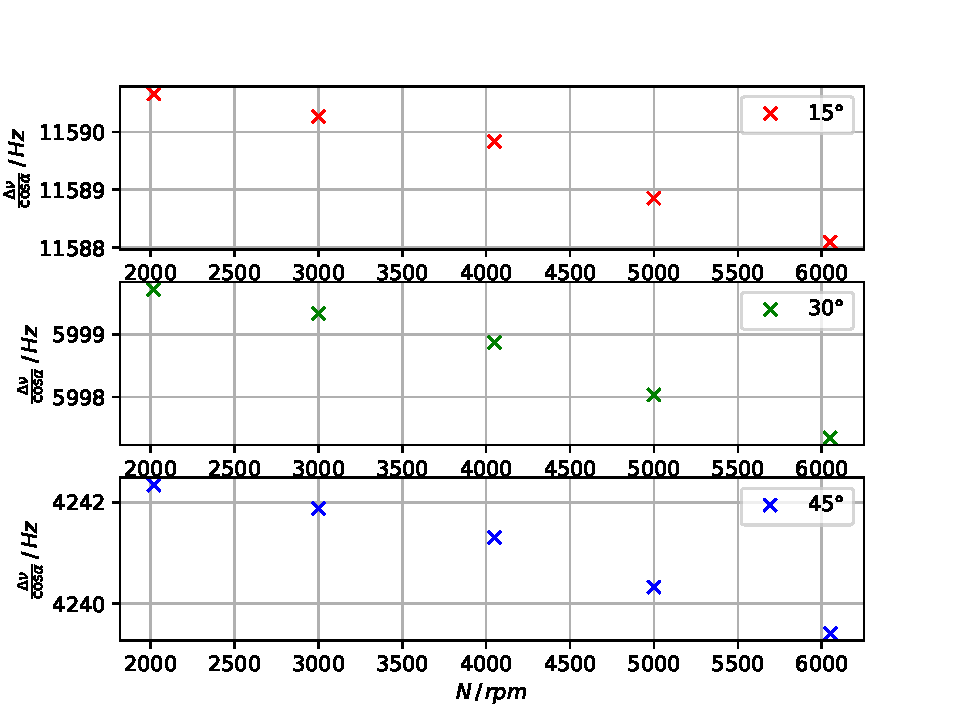
\includegraphics[width=\textwidth]{content/data/doppler.pdf}
    \caption{Die aufgenommenen Frequenz aufgetragen gegen die Umdrehungsgeschwindigkeit der Punmpe.}
    \label{fig:doppler}
\end{figure}

\FloatBarrier

Im nächsten Teil des Experiments wurde die Streuintensität $I$ sowie die maximale Frequenz $f_\text{max}$ des refelktierten Schalls in Abhängigkeit von der Messtiefe der Schallsonde gemessen.
Dafür wurden an der Sonde verschiedene Messtiefen in $\si{\micro\second}$ eingestellt.
Die so aufgenommnen Werte sind in Tabelle \ref{tab:depth} zu finden.
In dem linken Teil der Tabelle sind dabei die Messwerte für eine Umdrehungsgeschwindigkeit $N$ von $\SI{3880}{rpm}$ zu sehen und im rechtem Teil der Tabelle die Messwerte für $\SI{6000}{rpm}$.

\begin{table}
    \centering
    \begin{tabular}[t]{ccc}
    \toprule
    $Tiefe \,/\, \SI{}{\micro\second}$ & $I \,/\, \SI{}{100\frac{\volt^2}{\second}} $ & $f_\text{max}\,/\, \SI{}{\Hz} $\\
    12.5 & 93 & 400     \\
    13.0 & 130 & 430    \\
    13.5 & 200 & 500    \\
    14.0 & 207 & 502    \\
    14.5 & 215 & 514    \\
    15.0 & 160 & 490    \\
    15.5 & 160 & 457    \\
    16.0 & 300 & 420    \\
    16.5 & 301 & 380    \\
    17.0 & 190 & 400    \\
    17.5 & 155 & 400    \\
    18.0 & 184 & 390    \\
    18.5 & 196 & 400    \\
    19.0 & 225 & 430    \\
    \bottomrule
    \end{tabular}
    \begin{tabular}[t]{ccc}
    \toprule
    $Tiefe \,/\, \SI{}{\micro\second}$ & $I \,/\, \SI{}{100\frac{\volt ^2}{\second}} $ & $f_\text{max}\,/\, \SI{}{\Hz} $\\
    12.5 & 100 & 800        \\
    13.0 & 120 & 860        \\
    13.5 & 200 & 1020       \\
    14.0 & 235 & 1092       \\
    14.5 & 260 & 1185       \\
    15.0 & 350 & 1206       \\
    15.5 & 370 & 1225       \\
    16.0 & 400 & 1020       \\
    16.5 & 390 & 930        \\
    17.0 & 420 & 950        \\
    17.5 & 345 & 980        \\
    18.0 & 320 & 990        \\
    18.5 & 300 & 1100       \\
    19.0 & 260 & 1200       \\
    \bottomrule
    \end{tabular}
    \caption{Die Streuintensität und die maximale Frequenz des reflektierten Schalls in abhängigkeit der Messtiefe. Die Messwerte der linke Tabelle wurden bei $\SI{3880}{rpm}$ gemessen, die der rechten bei $\SI{6000}{rpm}$}
    \label{tab:depth}
\end{table}

Für eine graphische Auftragung der Messwerte wird zunächst die Messtiefe $s$ von $\si{\micro\second}$ in $\si{\milli\meter}$ umgerechnet.
Daür wird zunächst die Strecke $s_\text{prism}$ subtrahiert die der Schall im Prisma zurücklegt.
\begin{equation*}
 s_\text{liquid} = s - \frac{s_\text{prism}}{c_\text{prism}}
\end{equation*}
$c_\text{prism}$ enspricht dabei der Schallgeschwindigkeit im Prisma.
Daraufhin wird mit dem Weg-Zeit-Gesetzt
\begin{equation*}
l = c_\text{liquid} s,
\end{equation*}
die Messtiefe $s$, mithilfe der Schallgeschwindigkeit $c_\text{liquid}$ in der Flüssigkeit, in eine Distanz $l$ in $\si{\milli\meter}$ umgerechnet.
Gegen diese wird nun die Streuintensität $I$ und die maximale Frequenz $f_\text{max}$ graphisch aufgetragen.
Dabei sind die Abbildung für $N = \SI{3880}{rpm}$ und $N = \SI{6000}{rpm}$ getrennt.
Die graphisch aufgetragenen Messwerte für $N = \SI{3880}{rpm}$ sind in Abbildung \ref{fig:3880} zu sehen, die für $N = \SI{6000}{rpm}$ sind in der Graphik \ref{fig:6000} zu finden.

\begin{figure}
    \centering
    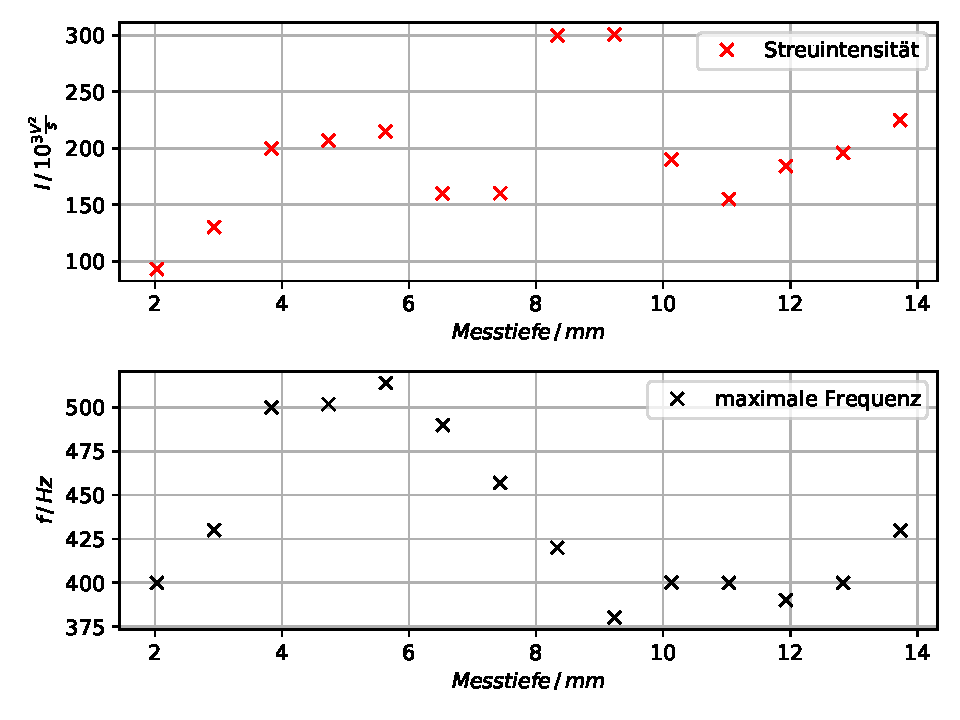
\includegraphics[width=\textwidth]{content/data/depth_3880.pdf}
    \caption{Die obere Graphik zeigt die Streuintensität aufgetragen gegen die Messtiefe, die untere die Frequenz aufgetragen gegen die Messtiefe. $N=\SI{3880}{rpm}$}
    \label{fig:3880}
\end{figure}

\begin{figure}
    \centering
    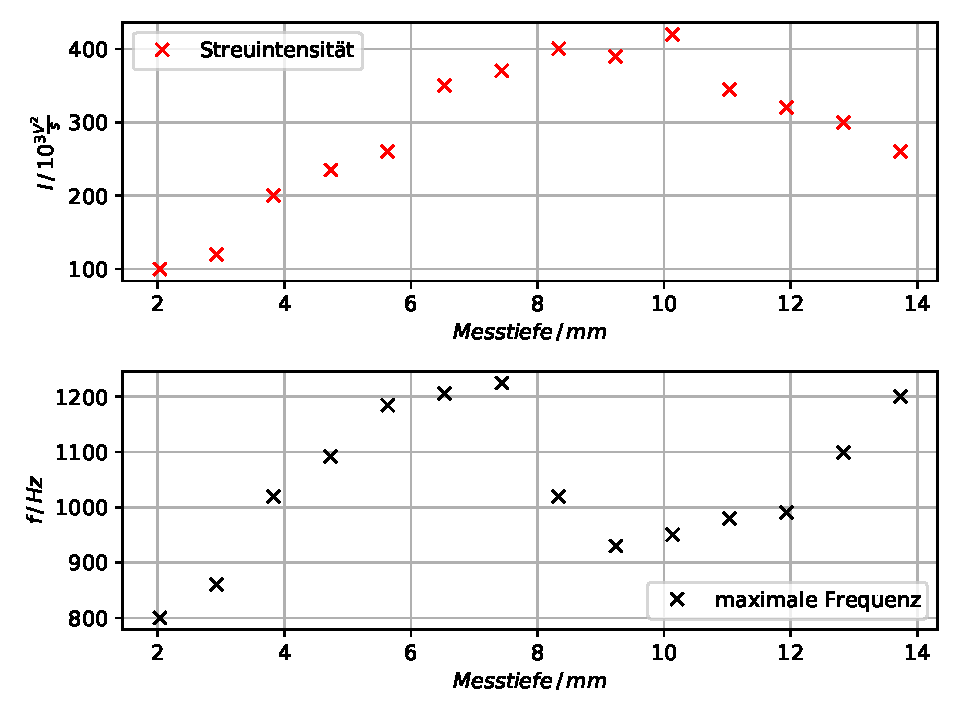
\includegraphics[width=\textwidth]{content/data/depth_6000.pdf}
    \caption{Die obere Graphik zeigt die Streuintensität aufgetragen gegen die Messtiefe, die untere die Frequenz aufgetragen gegen die Messtiefe. $N=\SI{6000}{rpm}$}
    \label{fig:6000}
\end{figure}
